% Summary results, v2 (final). Every number is read from FINAL_v2/v2_gridsearch/REPORT.md (run 2026-10-16 14:32, 31 datasets x 11 models)
% and the generated tables under paper/v2/tables/.  Compile from FINAL_v2/paper/ (tables resolve through \input@path) or as paper/v2/main.tex.
\documentclass[11pt]{article}
\usepackage[margin=1in]{geometry}
\usepackage{booktabs,graphicx,longtable,tabularx,array,caption,subcaption,amsmath,hyperref,enumitem,xcolor,pdflscape}
\usepackage[T1]{fontenc}
\usepackage{lmodern}
\captionsetup{font=small,labelfont=bf}
\setlist{nosep,leftmargin=*}
\newcolumntype{L}{>{\raggedright\arraybackslash}X}
\graphicspath{{figures/}{v2/figures/}}
\makeatletter\def\input@path{{./}{v2/}}\makeatother
\emergencystretch=1.5em
\newcommand{\notable}[1]{\par\noindent\begingroup\small\textbf{Notable.} #1\endgroup\par\medskip}
\newcommand{\inoneline}[1]{\par\noindent\begingroup\small\textit{In one line: #1}\endgroup\par\medskip}
\hypersetup{colorlinks=true,linkcolor=blue!60!black,citecolor=blue!60!black,urlcolor=blue!60!black}

\title{Summary Results}
\author{}
\date{2026}

\begin{document}
\maketitle

\section{Setup}
\label{sec:setup}

\subsection{Suite and pools}
\begin{itemize}
\item 31 datasets: 11 entity matching (EM), 6 schema matching (SM), 11 table question answering and understanding (TQA), 3 financial documents (FIN). Each adapter reads the official test or dev split and emits items with a question, a context (table, document, or record pair), a gold answer with aliases, a list gold where the answer is a set, an answer type (numeric / boolean / text / free-form) and the dataset's native metric.
\item Pools: 150 items per dataset by seeded stratified sampling (strata: question type, sub-task, database, product category, match label); 100 flagged for answering (OfficeQA Pro V2: all 90; Alaska schema: 93). The remaining 50 are a seeded reserve and are not used by any step. Total answered items: 3,083 per model.
\item Entity-matching pools are 50/50 match / non-match (Papadakis--Christen keeps its real 1.8\,\% match ratio). Schema matching is framed as one question per source column with a candidate list that always contains the gold. BIRD is graded on the executed result of the gold SQL, not on SQL text.
\item Official census: every dataset's official population is counted by the same strata, so that pool numbers can be re-weighted to the official split (Section~\ref{sec:setup:official}).
\end{itemize}

\subsection{Collecting answers}
\begin{itemize}
\item One prompt per item: context, question, and an answer-format line requesting \texttt{FINAL ANSWER: <answer>}.
\item Models (eleven): Claude Opus 5, Claude Sonnet 5, GPT-5.5, GPT-5.4-mini, Gemini 3.1 Pro, Gemini 3.8 Flash, Grok 4, DeepSeek-chat, DeepSeek-R1, gpt-oss-120b (Together), Llama 3.3 70B (Together). Gemini 3.1 Pro was collected over three weeks under Google's daily quota (a scheduled GitHub Actions workflow plus a final local run) and entered the study once it passed the 90\,\% coverage rule.
\item Decoding: temperature 0 where the API accepts it (Gemini, Grok, DeepSeek, Llama, gpt-oss). Claude 5 reports the parameter deprecated and GPT-5.5 rejects any non-default value; those ran at provider defaults. Every cached row records which applied.
\item Output budget 700 tokens. A reply cut off for length with no final-answer line is re-asked at 2,500 tokens, then 8,000, then 16,000 (and 32,000 for the two Claude Sonnet 5 replies still unfinished at 16,000). The trigger is mechanical (finish reason plus absence of the final line), never correctness. Originals are archived with a reason; replacement rows carry \texttt{attempt} = 2 to 5. The budget is counted in each provider's own tokens and, for the reasoning models, includes their chain of thought, so it is a termination test rather than an equal text allowance. Replies still unfinished at the last stage are scored as given (effectively failures): 41 DeepSeek-R1 answers at 16,000 tokens, plus 123 DeepSeek-R1 answers whose 16,000-token re-ask is pending on provider balance and stand at their 8,000-token replies.
\item Every answer is cached with tokens, latency, cost, finish reason and decoding; re-runs skip cached items. Cost: USD 174 for the answers in the final cache (Claude Opus 5: USD 107 including its re-asks; Gemini 3.1 Pro: USD 12), USD 224 over the whole project including the archived truncated originals.
\end{itemize}

\subsection{Scoring an answer}
\begin{itemize}
\item Extraction: the \texttt{FINAL ANSWER:} line; else a boxed expression; else the last short line of the reply.
\item Normalisation: Unicode NFKC, lower-case, canonical numbers (``1,577.00'' $\to$ ``1577'', ``(12.6)'' $\to$ ``$-$12.6''), currency symbols and punctuation removed, articles dropped, whitespace collapsed.
\item Units and scale: every number is parsed with sign, percent marker (\%, ``percent'', ``pp'') and scale word (thousand / million / billion / trillion and abbreviations). A parsed number exposes its equivalent readings (raw, scaled, $\div 100$ if marked percent, $\times 100$ if an unmarked fraction); the relative error between prediction and gold is the minimum over all pairs of readings. Real-unit conversions (km $\leftrightarrow$ miles) are not attempted.
\item Aliases: each item carries the primary gold plus acceptable alternatives supplied by the adapter (e.g.\ \emph{yes} $\equiv$ \emph{match} $\equiv$ 1; several legitimate target columns in schema matching; comma- and pipe-joined forms of list golds). Every component is computed against each alias and the best-scoring alias is kept. Booleans are canonicalised before comparison.
\item Components per answer: token F1, numeric decay $e^{-2.5\cdot\text{rel.\ err}}$ (error clipped at 2; falls back to exact match for non-numeric golds), token precision, token recall; also exact match, numeric tolerance (1\,\%), ROUGE-L, and a hedge flag (several distinct numeric candidates, ``A or B'', or an enumeration of short candidates).
\item Native metric per dataset (baseline column): numeric tolerance for numeric golds, exact match for text and boolean golds, ROUGE-L for free-form (FeTaQA).
\item Composite under weighting $w$ on the simplex: $R_w = \sum_k w_k m_k$, $k \in \{$F1, decay, precision, recall$\}$. v1 is $w = (0.35, 0.35, 0.15, 0.15)$.
\item Dataset score of a model: mean $R_w$ over the items that every model answered. A model is in the study only if it covered $\ge 90\,\%$ of the suite; a dataset is used only with $\ge 20$ answered items.
\end{itemize}

\subsection{Evaluating a weighting}
\begin{enumerate}
\item \textbf{Agreement $J(w)$.} Rank the eleven models inside each dataset under $w$; pool the 31 rankings by Borda; $J$ is the mean Kendall $\tau_b$ between each dataset's ranking and the pooled one. $J$ measures consistency between datasets, not correctness. Computed for all 1,771 weightings of the step-0.05 simplex lattice (v1, the four corners and the uniform mix are lattice points), and also under Kemeny, Copeland and Bradley--Terry pooling.
\item \textbf{Correctness $\rho(w)$.} 31,380 synthetic answers of known utility generated from the golds of the answered items by typed operators (identity, alias, unit variant, typo, rounding, magnitude error, sign flip, wrong value, partial list, superset, hedge, verbose, no answer, \dots). Reported: Spearman $\rho$ between $R_w$ and utility, AUC correct vs wrong, mean score of wrong answers, hedge gap; the $(J,\rho)$ Pareto front and its knee.
\item \textbf{Honest selection.} Nested item bootstrap ($B=1{,}000$): choose the best $w$ on in-bag items, score it out of bag. Reported: the optimism gap, the paired out-of-bag difference to v1 with a 95\,\% interval, and the plateau (weightings not significantly below the best, paired bootstrap $p>.05$) plus a practical plateau (within 0.02 of the best).
\item \textbf{Transfer.} Leave-one-dataset-out and leave-one-family-out: re-fit $w$ on the rest, measure $\tau$ of the held-out dataset's ranking to the pooled rest; per-family optima; sensitivity to one lattice step (0.05).
\item \textbf{Designs.} Uniform-lattice, Dirichlet-snapped and Latin-hypercube samples of 100 weightings, 20 seeds each, compared with the exhaustive optimum (regret, rank of the found best, centred $L_2$ discrepancy, minimum pairwise $L_1$).
\end{enumerate}

\subsection{From scores to a leaderboard}
\label{sec:setup:official}
\begin{itemize}
\item Rules reported: exact match only, v1, the five best by $J$, the best by $\rho$, the $(J,\rho)$ Pareto knee.
\item Pooling: Bradley--Terry strengths from item-level pairwise wins (MLE, ridge 0.01, standard errors from the observed information) as the headline; Borda, mean-$z$, Kemeny (with cost), Copeland, reciprocal-rank fusion and family-balanced $z$ as checks.
\item Uncertainty: 1,000 item bootstraps of the Borda and Bradley--Terry rankings (rank intervals, probability of first place), saved in full.
\item Significance: Friedman with the Iman--Davenport correction across datasets, Nemenyi critical difference, Holm-corrected pairwise Wilcoxon; paired permutation and Wilcoxon per dataset and model pair (Holm within dataset); Kendall's $W$ among datasets; majority-class baselines for boolean sets.
\item Official-split estimates: the same answers re-weighted by official stratum share / sample share (post-stratification) with a weighted item bootstrap; positive-class precision, recall and F1 at the official match ratio for the matching sets.
\item Diagnostics: pairwise $\tau$ between dataset rankings; floor, ceiling and self-stability flags per dataset.
\item Reporting: one script regenerates the report from the cached answers in minutes, so text and numbers cannot disagree.
\end{itemize}

\section{Results}
\label{sec:results}

All numbers are from the run of 2026-10-16 (31 datasets $\times$ 11 models, 3,083 answered items per model). Table~\ref{tab:summary} gives the audit in one place; the subsections that follow give one figure or table per row.

\begin{table}[htbp]
\centering\small
\caption{Audit summary. $J$ = agreement objective (mean Kendall $\tau_b$ of each dataset's model ranking to the Borda pool); $\rho$ = Spearman correlation of the composite with known utility on 31,380 synthetic anchors.}
\label{tab:summary}
\begin{tabularx}{\textwidth}{>{\bfseries}p{0.30\textwidth} L}
\toprule
Exhaustive grid & 1,771 weightings (step 0.05); best F1 .35 / decay .60 / precision .05 / recall 0, $J=0.414$; v1 $J=0.392$ (rank 1,602 of 1,771) \\
$J$ over the lattice & range 0.376--0.414; median 0.401, 90th percentile 0.407, 99th percentile 0.412: a flat landscape \\
Plateau (paired bootstrap $p>.05$ vs best) & 1,749 of 1,771 (v1 inside, $p=0.63$); practical plateau within 0.02: 1,731 \\
Nested selection ($B=1{,}000$) & in-bag $J$ of the selected weighting 0.370, out-of-bag 0.323 (optimism gap 0.047); v1 out-of-bag 0.330 \\
Selected vs v1, out of bag & $-0.007$, 95\,\% CI $[-0.033,\,+0.011]$, $p=0.72$; 624 distinct weightings selected across resamples \\
Sampled designs (100 points, 20 seeds) & Dirichlet / LHS / uniform all reach $0.412$--$0.413\pm0.001$, regret $\le 0.004$: sampling would have sufficed \\
Objective under other pooling rules & Kemeny, Copeland and Bradley--Terry each pick a different ``best''; v1's rank swings from 615 (Bradley--Terry) to 1,602 (Borda): rank is noise \\
Transfer (leave-one-dataset-out) & held-out $\tau$: re-fitted weights $+0.33$, full best $+0.35$, v1 $+0.32$ \\
Leave-one-family-out & v1 within 0.05 of the held-out-fitted weights in every family (EM $+0.32$ vs $+0.32$, SM $+0.28$ vs $+0.33$, TQA $+0.33$ vs $+0.33$, FIN $+0.44$ vs $+0.45$) \\
Anchors (31,380 synthetic answers) & v1 $\rho=0.878$, best-$\rho$ weighting 0.883, best-$J$ weighting 0.876, exact match 0.828; AUC correct-vs-wrong 0.994 for every rule \\
$J$ vs $\rho$ across the lattice & $-0.23$ (was $-0.34$ at ten models and $+0.38$ on the 2,500-token cache): unstable because $J$ is flat; Pareto front of 17, knee = best $J$ \\
Sensitivity & one 0.05 step moves $J$ by at most 0.012 around v1 and 0.017 around the best \\
Leaderboard & Friedman $p<0.001$ under every rule; Kendall's $W$ among datasets 0.26--0.27 \\
Significant pairs (Holm, v1) & 15 of 55: nine models $>$ Llama 3.3 70B; Opus, GPT-5.5, Gemini 3.1 Pro, Gemini 3.8 Flash, DeepSeek-R1 and Grok 4 $>$ gpt-oss-120b \\
First place & Bradley--Terry: Gemini 3.8 Flash under v1 and every calibrated rule ($P(\text{first})$ 0.91--0.95), Claude Opus 5 under exact match (0.79); Borda: GPT-5.5 under v1 and the calibrated rules, Opus under exact match \\
Gemini 3.1 Pro & enters fifth by Bradley--Terry under v1 (fourth under exact match), below Flash, Opus, GPT-5.5 and Sonnet \\
Official-split comparability & accuracy moves by $\le 0.09$ after post-stratification (OpenSanctions); positive-class F1 on the balanced pools overstates official-ratio F1 by up to 0.19 (Amazon--Google) \\
Datasets at ceiling & Valentine, WDC LSPC, WDC Products (means 0.98): flagged; still inside the objective \\
Cost & USD 174 for the final cache (Opus 107); USD 224 over the project including archived truncated originals \\
\bottomrule
\end{tabularx}
\end{table}

\subsection{The objective is flat}
\inoneline{Every weighting of the four ingredients gives nearly the same agreement; v1's low rank is a rank inside noise.}
Figure~\ref{fig:landscape} shows $J$ for all 1,771 weightings. The whole lattice spans 0.376--0.414. The best weighting (F1 0.35, decay 0.60, precision 0.05) reaches 0.414 and v1 reaches 0.392; 1,601 weightings are nominally better than v1, but the entire spread is smaller than the bootstrap noise of a single weighting (about 0.027). No single weight has a slope worth acting on (Figure~\ref{fig:marginals}); the four ingredients correlate at 0.91--0.98 with one another and in 82\,\% of answers all four equal exact match, which is the mechanical reason.

\begin{figure}[htbp]
\centering
\begin{subfigure}{0.48\textwidth}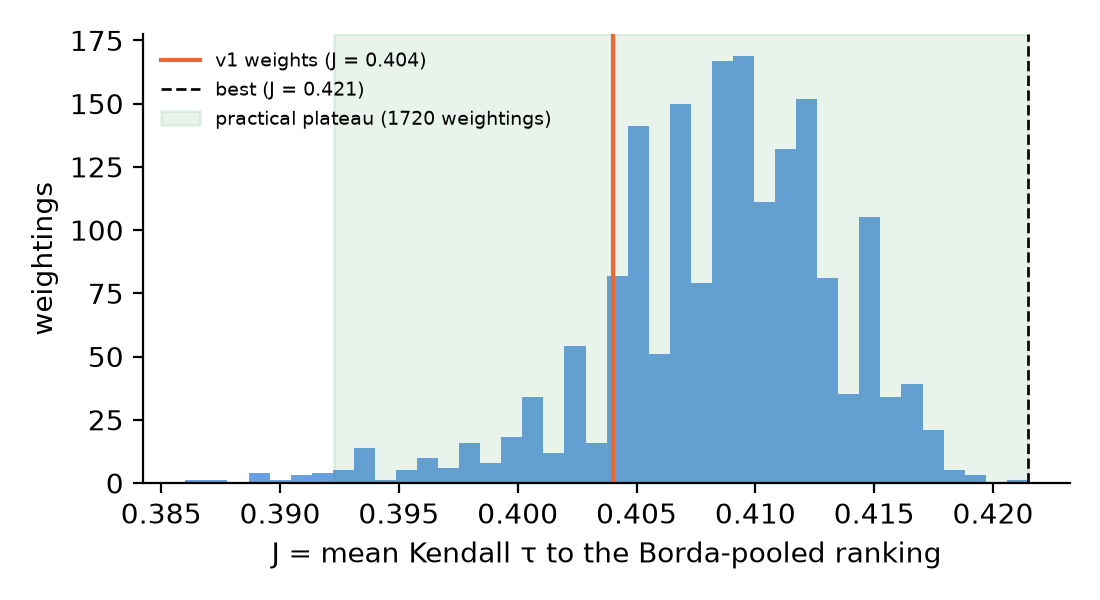
\includegraphics[width=\linewidth]{fig_j_histogram.png}\caption{Distribution of $J$ over the lattice with v1, the best and the plateau band.}\end{subfigure}\hfill
\begin{subfigure}{0.48\textwidth}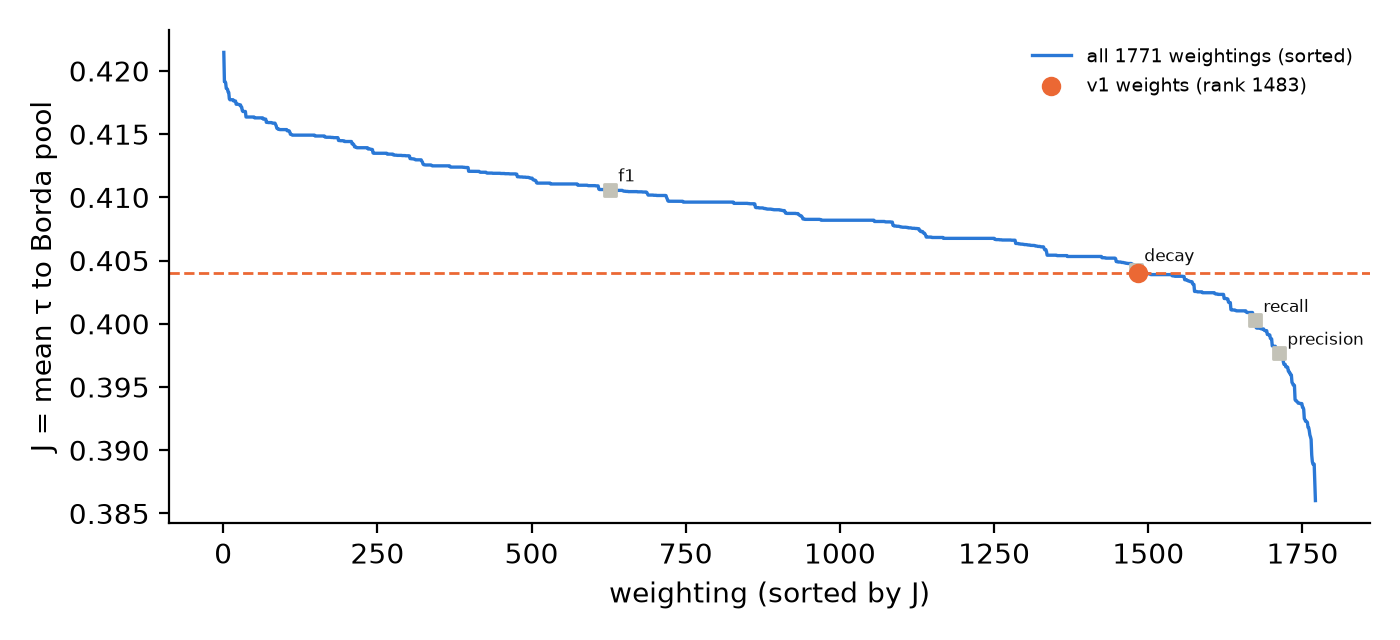
\includegraphics[width=\linewidth]{fig_landscape.png}\caption{Sorted $J$ with v1 and the four single-ingredient corners.}\end{subfigure}
\caption{The agreement landscape over all 1,771 step-0.05 weightings.}
\label{fig:landscape}
\end{figure}
\notable{(a) The histogram is narrow: 1,771 weightings fit between 0.376 and 0.414, and v1 (0.392) sits in the main body, not in a tail. (b) The sorted curve is flat for 1,700 weightings and only drops at the single-ingredient corners; v1's rank of 1,602 is a position on a plateau, which is why the report never quotes rank as a result.}

\begin{figure}[htbp]
\centering
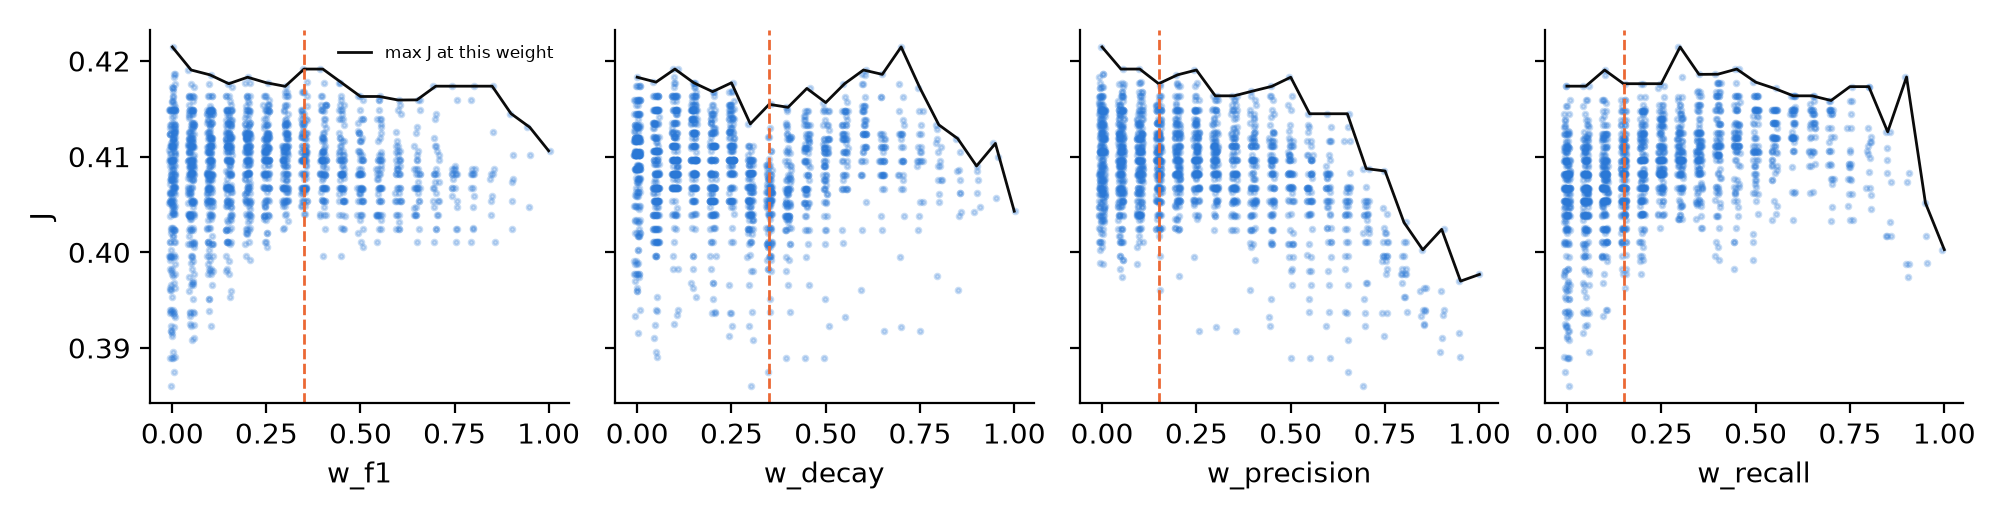
\includegraphics[width=0.95\textwidth]{fig_marginals.png}
\caption{$J$ against each of the four weights. Corners: F1 only 0.409, decay only 0.394, precision only 0.386, recall only 0.389; uniform 0.401.}
\label{fig:marginals}
\end{figure}
\notable{No panel has a slope worth acting on: the mean line moves by at most 0.018 across the full range of any weight (precision, falling as it approaches 1). The vertical scatter at every weight level, caused by the other three weights, is wider than any slope, so no ingredient can be tuned in isolation.}

\subsection{The best weighting does not survive honest selection}
\inoneline{Chosen honestly, the best weighting is no better than v1; 624 different weightings win depending on which items are drawn.}
Figure~\ref{fig:nested} reports the nested item bootstrap. The weighting chosen on in-bag items scores 0.370 in bag but 0.323 out of bag (optimism gap 0.047), below v1's out-of-bag 0.330. The paired out-of-bag difference to v1 is $-0.007$ with a 95\,\% interval of $[-0.033, +0.011]$ ($p=0.72$); the selected weighting is ahead of v1 in 28\,\% of resamples, and 624 distinct weightings were selected across the 1,000 resamples. The plateau of weightings not significantly below the best contains 1,749 of 1,771 points and v1 is inside it ($p=0.63$).

\begin{figure}[htbp]
\centering
\begin{subfigure}{0.48\textwidth}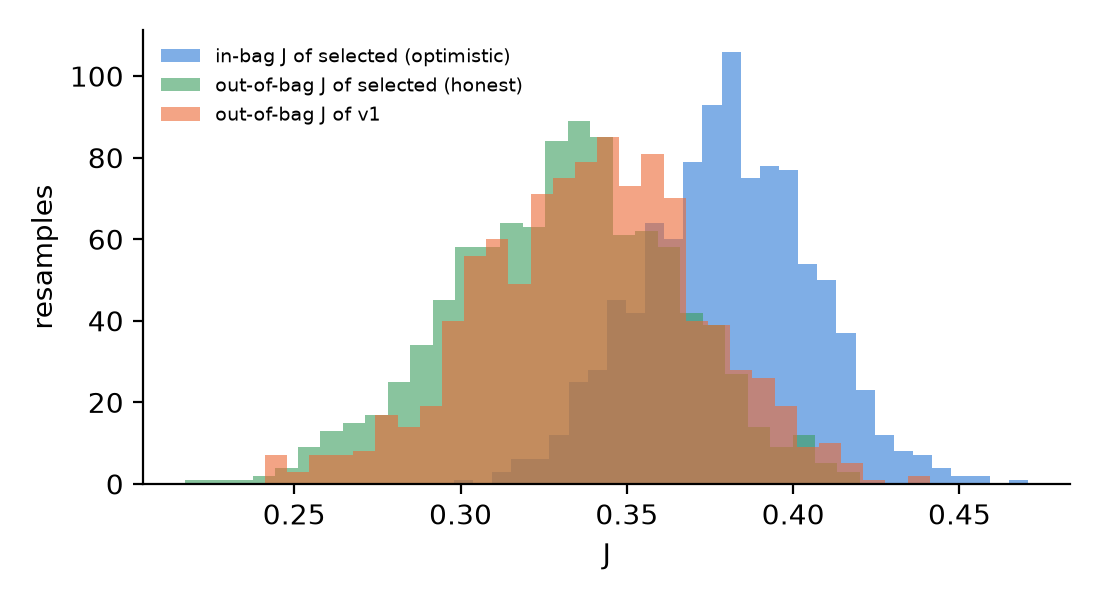
\includegraphics[width=\linewidth]{fig_nested.png}\caption{In-bag vs out-of-bag $J$ of the selected weighting against v1.}\end{subfigure}\hfill
\begin{subfigure}{0.48\textwidth}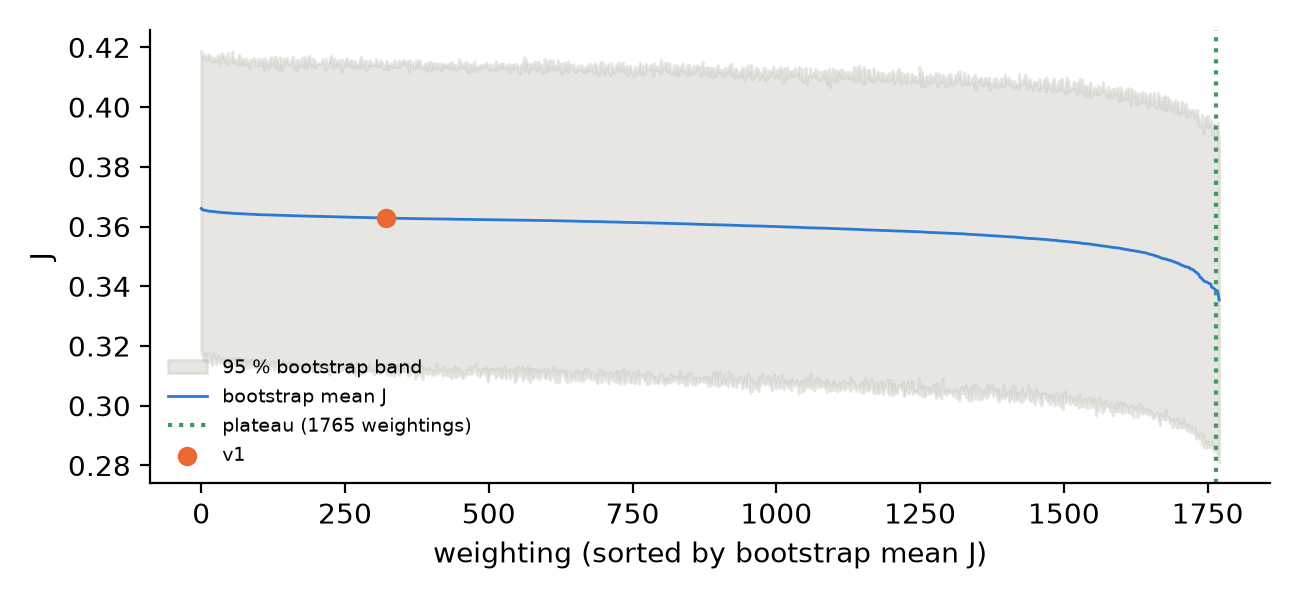
\includegraphics[width=\linewidth]{fig_plateau.png}\caption{Bootstrap band over sorted weightings; the plateau boundary.}\end{subfigure}
\caption{Honest selection: the optimism gap and the plateau.}
\label{fig:nested}
\end{figure}
\notable{(a) The in-bag winner looks 0.047 better than it is; out of bag it scores 0.323 against v1's 0.330, and the paired difference of $-0.007$ has a 95\,\% interval through zero. (b) 1,749 of 1,771 weightings are inside the plateau and v1 is one of them ($p = 0.63$); the only points outside are decay-dominated corners with no F1 or recall.}

\input{tables/designs_short.tex}
\notable{All three 100-point designs reach 0.412--0.413 with a worst-seed regret of 0.004 against the exhaustive 0.414. With four weights the exhaustive grid costs nothing, so the table matters only as evidence that sampling would have sufficed in the larger sibling searches.}

\begin{figure}[htbp]
\centering
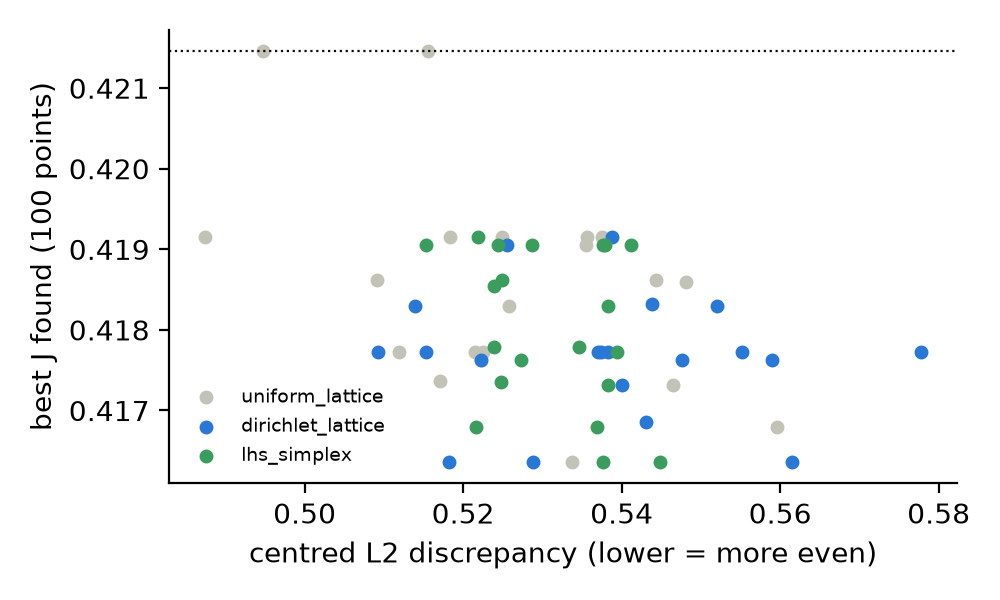
\includegraphics[width=0.8\textwidth]{fig_designs.png}
\caption{Any 100-point design finds the plateau; regret against the exhaustive optimum is at most 0.004.}
\label{fig:designs}
\end{figure}


\subsection{The optimum does not transfer, and neither does the rank}
\inoneline{Re-fitted weights predict a held-out dataset no better than v1, and families want different weights.}
Leave-one-dataset-out: weights re-fitted without the held-out dataset predict its ranking with mean $\tau=+0.33$, the full-data best with $+0.35$, v1 with $+0.32$ (Table~\ref{tab:lofo_short} gives the family-level version). Per-family optima pull in different directions (Figure~\ref{fig:family}): decay-only for schema matching, recall-heavy for table QA and finance, F1-and-decay for entity matching, yet none is far from the plateau. Changing only the pooling rule inside the objective moves v1's rank from 615 (Bradley--Terry) to 1,602 (Borda) and changes which weighting is ``best'', so rank inside a flat objective carries no information.

\input{tables/lofo_short.tex}
\notable{Held-out $\tau$ under re-fitted weights is within 0.05 of v1 in every family (EM $+0.32$ vs $+0.32$, SM $+0.33$ vs $+0.28$, TQA $+0.33$ vs $+0.33$, FIN $+0.45$ vs $+0.44$). The re-fitted weights themselves swing from F1-heavy (EM) to recall-heavy (SM) to decay-heavy (FIN): there is no single weighting the families agree on.}

\begin{figure}[htbp]
\centering
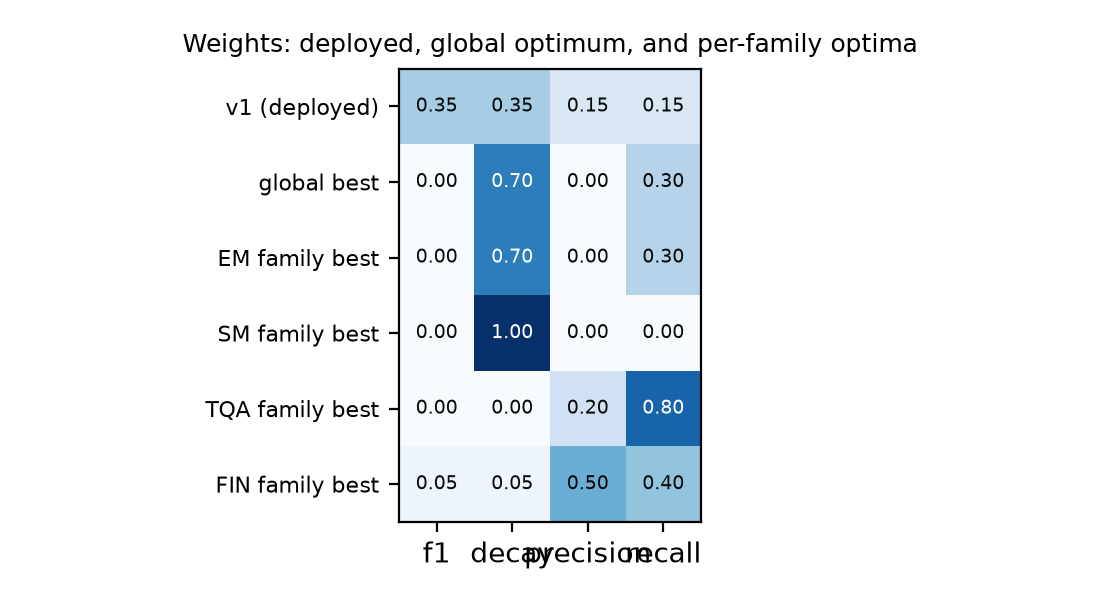
\includegraphics[width=0.85\textwidth]{fig_family_weights.png}
\caption{Deployed weights (v1), the global optimum and the per-family optima.}
\label{fig:family}
\end{figure}
\notable{Schema matching wants decay only, table QA and finance want recall-heavy mixes, entity matching wants F1 and decay; the global optimum is a compromise between them, and v1 is another. The suite-level flatness is partly these pulls cancelling, which is also why leave-one-family-out re-fits land far from the global best without doing better on the held-out family.}

\subsection{Agreement and correctness do not pull the same way}
\inoneline{Agreement among datasets and correctness on known answers are different criteria; v1 is near the correctness optimum.}
On 31,380 synthetic answers of known utility, v1 scores $\rho=0.878$; the best weighting by $\rho$ reaches 0.883 and the best by $J$ 0.876; exact match 0.828. Every rule separates correct from wrong answers with AUC 0.994. Across the lattice $J$ and $\rho$ correlate $-0.23$ on this cache, $-0.34$ at ten models and $+0.38$ on the earlier 2,500-token cache, which is what a flat $J$ predicts. With eleven models the Pareto knee coincides with the best-$J$ weighting (Table~\ref{tab:anchors_rules}, Figure~\ref{fig:pareto}).

\input{tables/anchors_rules.tex}
\notable{v1 scores $\rho = 0.878$, within 0.005 of the best attainable 0.883; the best-by-$J$ weighting is 0.876 and exact match 0.828. Every rule has AUC 0.994: all separate right from wrong, and they differ only in partial credit for near misses, unit variants and partial lists.}

\begin{figure}[htbp]
\centering
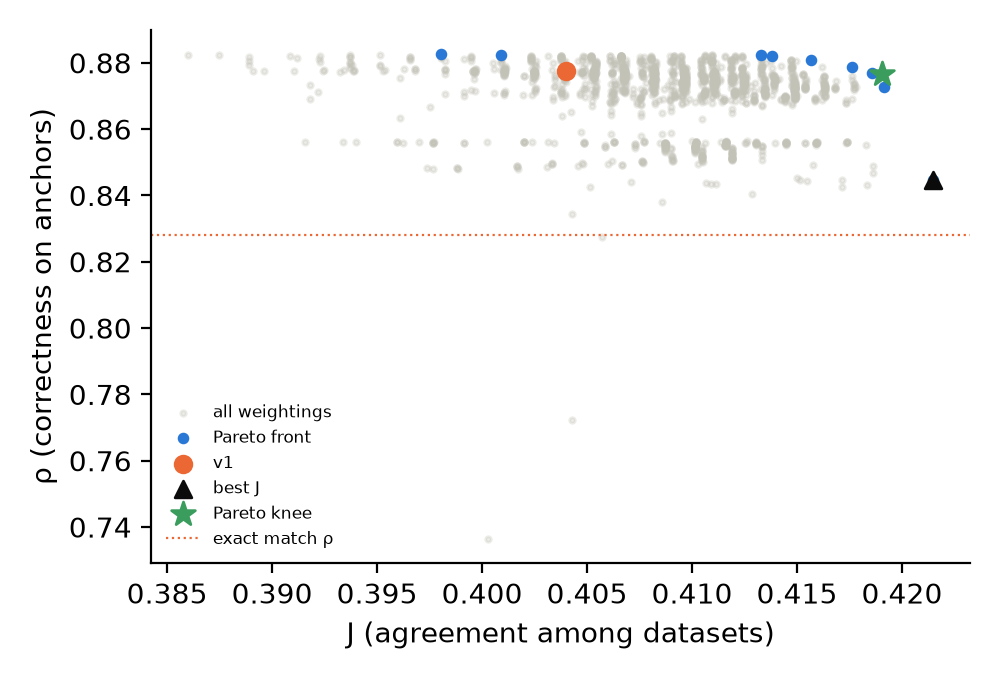
\includegraphics[width=0.75\textwidth]{fig_pareto.png}
\caption{Agreement $J$ against anchor correctness $\rho$ for every weighting; v1, the best-$J$, best-$\rho$ and knee points marked.}
\label{fig:pareto}
\end{figure}
\notable{The cloud is wide in $\rho$ (0.74--0.88) and narrow in $J$ (0.38--0.41), and the two correlate $-0.23$: agreement is not a proxy for correctness. v1 sits on the upper edge near the $\rho$ optimum; recall-only and decay-only, the corners that score well on $J$, are the worst by $\rho$.}

\subsection{Leaderboard}
\inoneline{The ends of the table are certain, the top three reorder with the rule, and Gemini 3.1 Pro lands fifth.}
Under every rule the Friedman test rejects equal models ($p<0.001$) while datasets agree only moderately (Kendall's $W$ 0.26--0.27). The ends of the ranking are stable: Llama 3.3 70B is last and gpt-oss-120b tenth under every rule and every pooling method, with Holm-corrected significance against the top group. The order inside the top three depends on the rule and the pooling method (Tables~\ref{tab:leaderboard_headline} and \ref{tab:ranks_by_rule}, Figure~\ref{fig:leaderboard}): Bradley--Terry puts Gemini 3.8 Flash first under v1 and all calibrated rules, Borda puts GPT-5.5 first under those rules, and exact match puts Claude Opus 5 first under both. Gemini 3.1 Pro, added in this run, lands fifth by Bradley--Terry under v1 and fourth under exact match; DeepSeek-R1 moved up one place after its unfinished answers were re-asked at 16,000 tokens.

\input{tables/leaderboard_headline.tex}
\notable{Gemini 3.8 Flash is first by Bradley--Terry with $P(\text{first}) = 0.91$ because it wins many items by small margins; by Borda, which counts dataset-level ranks, GPT-5.5 is first and Flash third. The bottom two (gpt-oss-120b, Llama 3.3 70B) have rank intervals of width zero; ranks 4--9 overlap and are not established.}
\input{tables/ranks_by_rule.tex}
\notable{Rows 10 and 11 never move; the top three permute with the rule (exact match favours Opus, every graded rule favours Flash by Bradley--Terry and GPT-5.5 by Borda). Gemini 3.1 Pro is fourth or fifth under every rule (fourth under exact match and the second to fourth $J$ weightings, fifth otherwise); DeepSeek-R1 sits fifth to eighth, seventh under v1, after its 16,000-token re-asks. Kendall's $W$ among datasets is 0.26--0.27 under every rule.}

\begin{figure}[htbp]
\centering
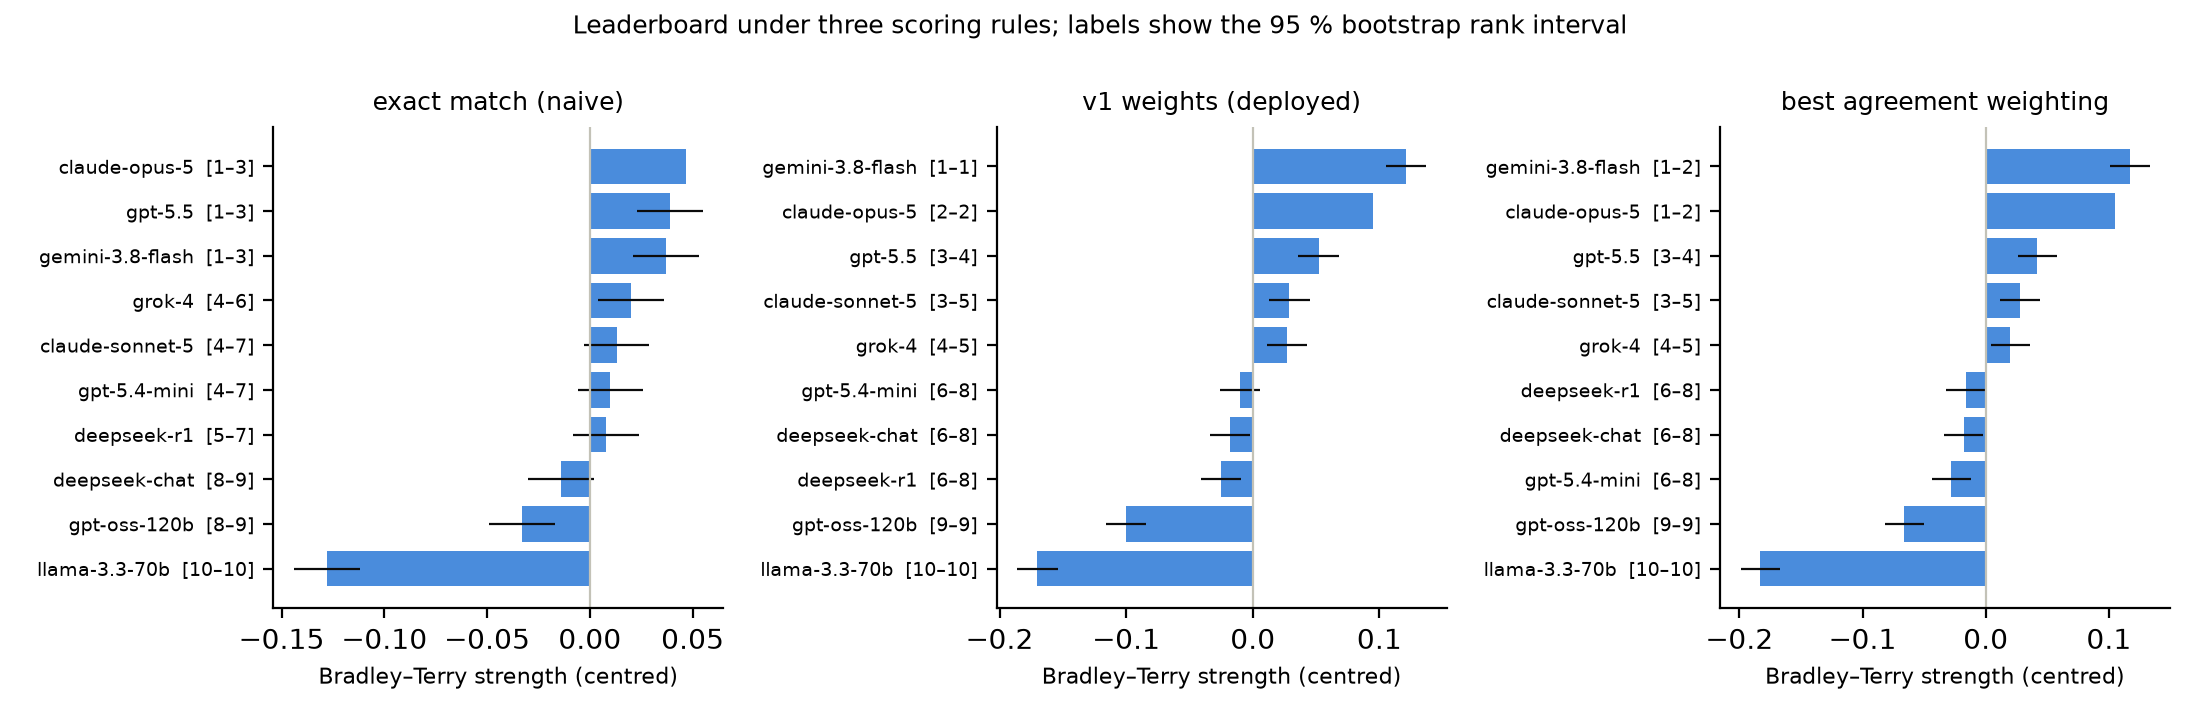
\includegraphics[width=0.95\textwidth]{fig_leaderboard_rules.png}
\caption{Bradley--Terry strengths $\pm$ SE with bootstrap rank intervals under exact match, v1 and the best-$J$ weighting. The ends are stable; the top order is rule-dependent.}
\label{fig:leaderboard}
\end{figure}
\notable{The strengths of ranks 4--9 lie within about 0.05 of each other with overlapping error bars; the gap from rank 9 to rank 10 and from 10 to 11 is larger than the whole middle band. The figure is the visual form of the Holm result: 15 of 55 pairs significant, all of them against the bottom two models.}

\begin{figure}[htbp]
\centering
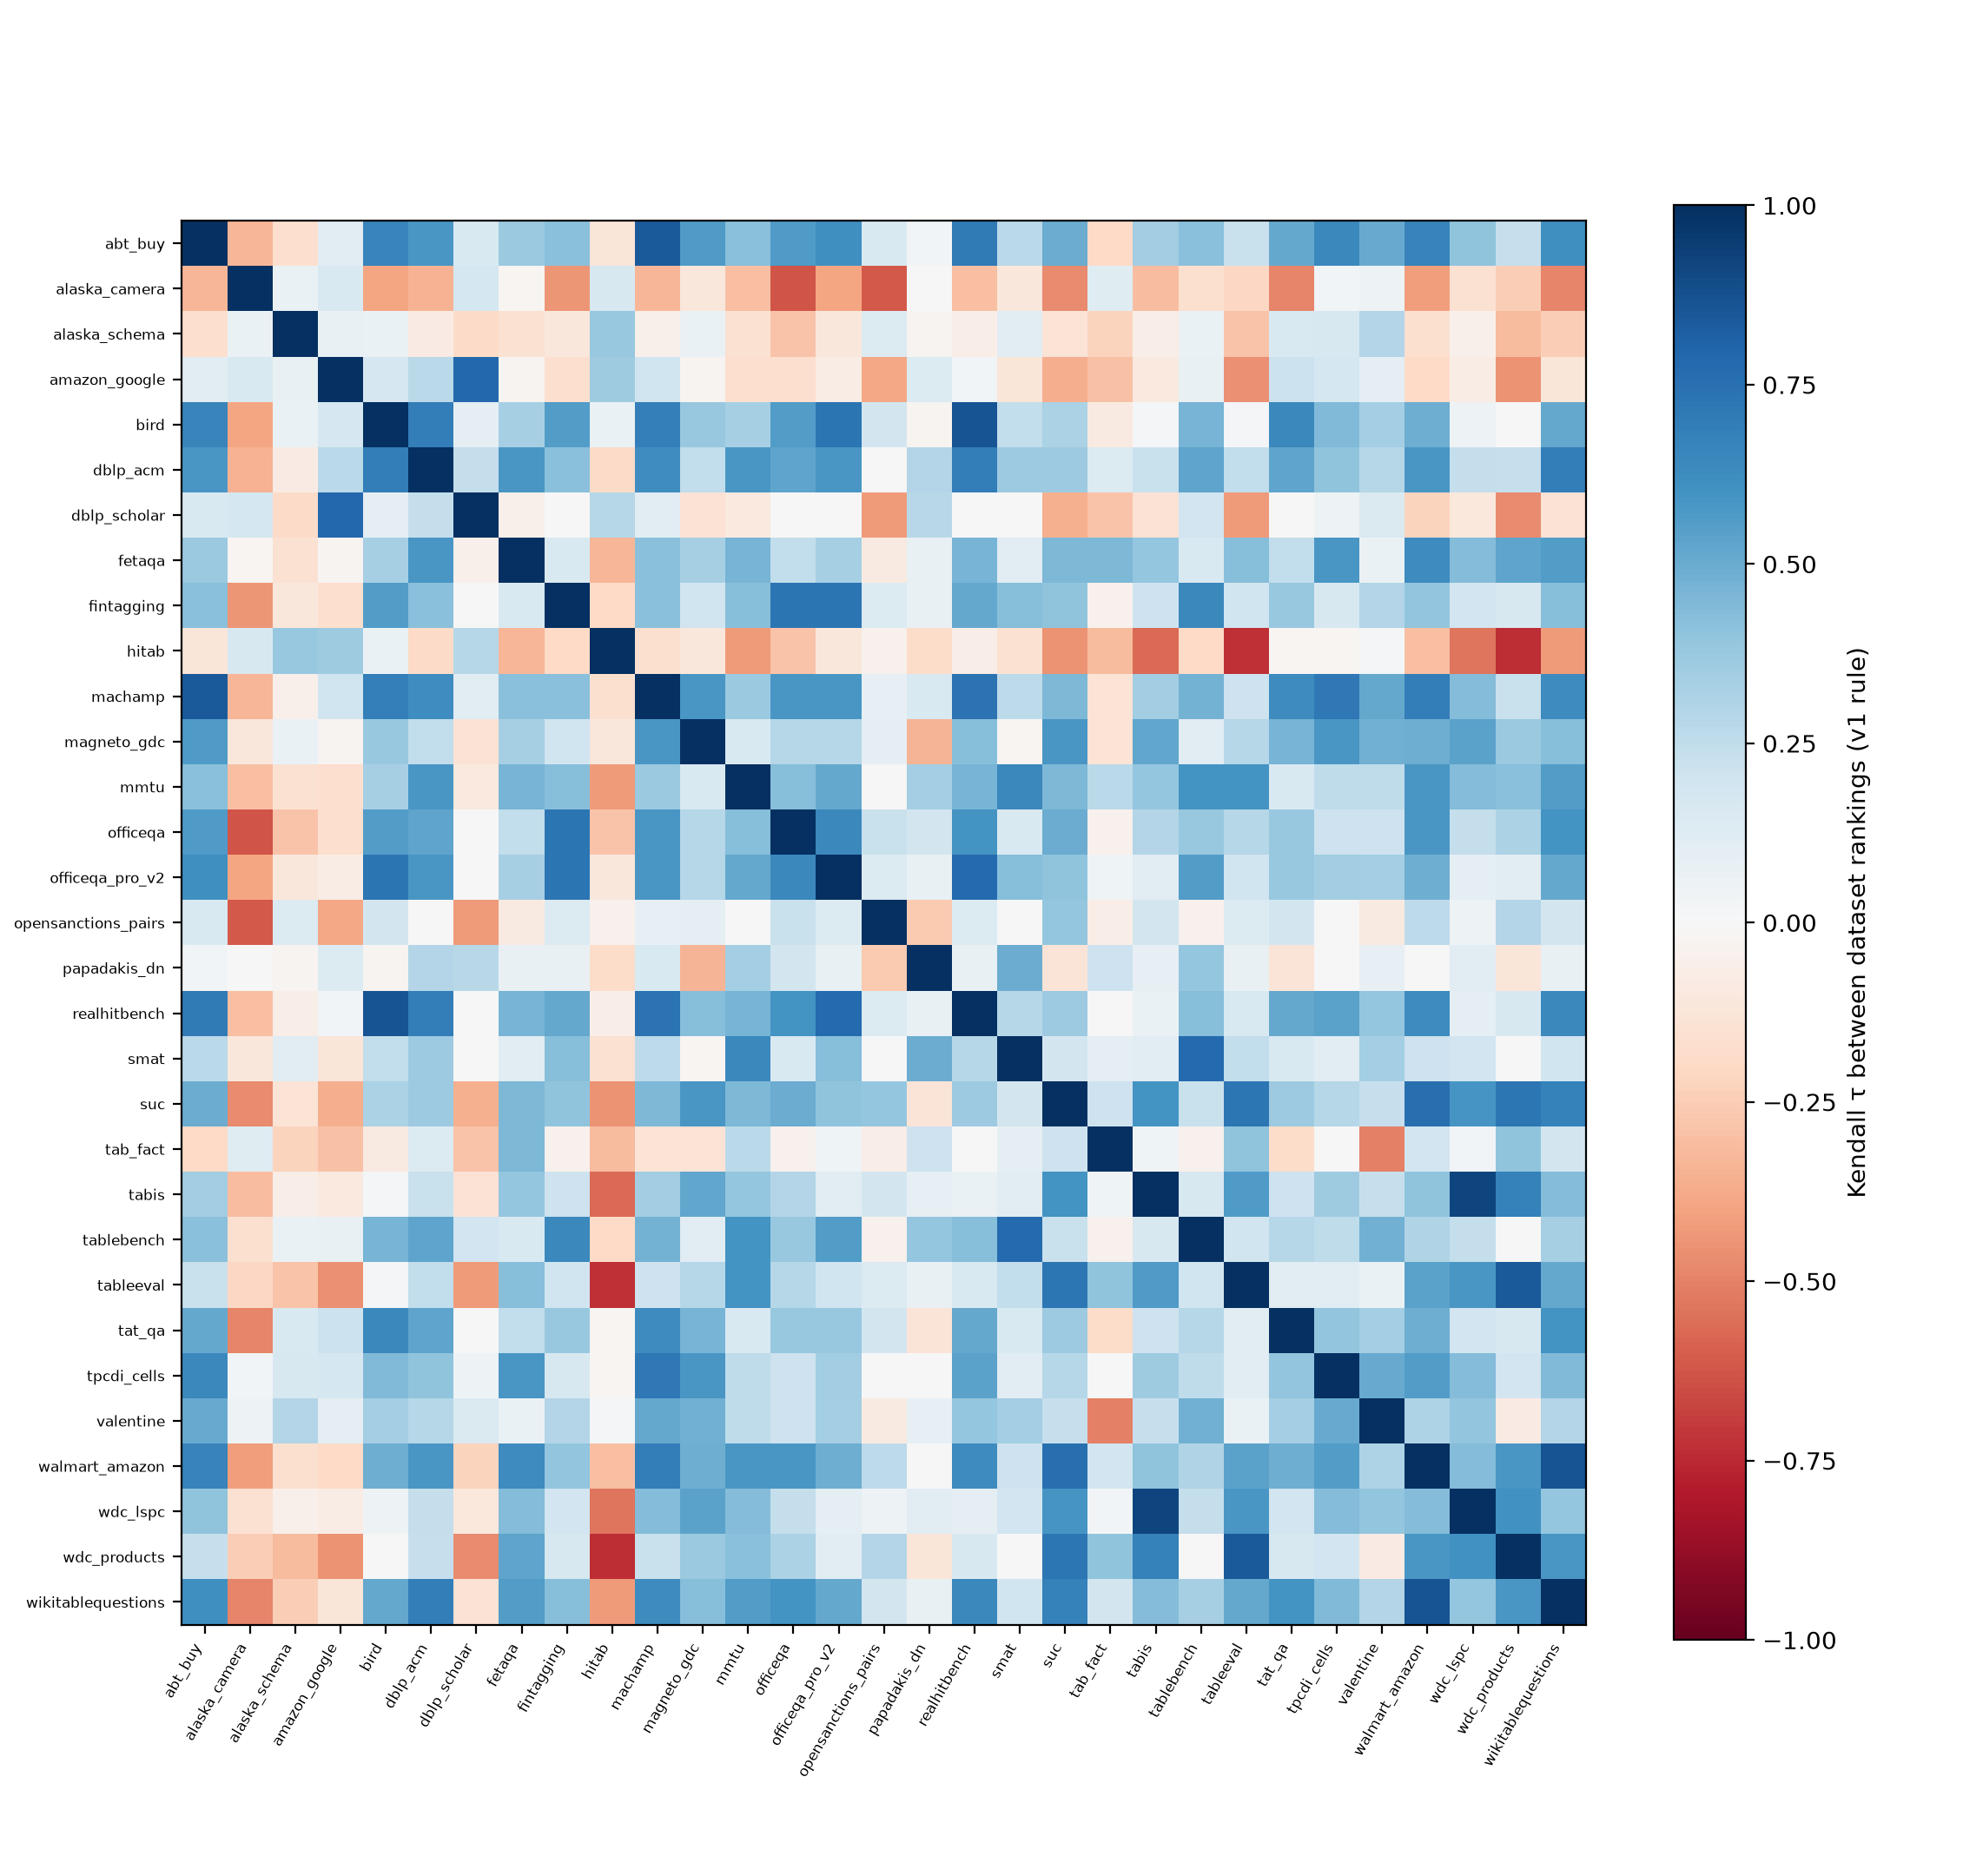
\includegraphics[width=0.8\textwidth]{fig_dataset_tau.png}
\caption{Kendall $\tau$ between the model rankings of each pair of datasets under v1. Datasets agree only moderately ($W\approx0.26$).}
\label{fig:dataset_tau}
\end{figure}
\notable{Blue blocks sit inside families and the finance and table-QA sets agree with most of the suite; Alaska Camera and HiTab are red against almost everyone. The leaderboard is an average over datasets that disagree about the middle of the table, which is what $W = 0.26$ says in one number.}

\subsection{Comparability with published numbers}
\inoneline{Accuracy survives re-weighting to the official splits; balanced-pool F1 on sparse matching sets does not.}
Post-stratification to the official split changes dataset accuracy by at most 0.09 (OpenSanctions pairs). For the matching sets, positive-class F1 computed on the balanced 50/50 pool overstates F1 at the official match ratio wherever the official split is sparse, by up to 0.19 on Amazon--Google (Table~\ref{tab:official_split_by_dataset}, Figure~\ref{fig:official}).

\input{tables/official_split_by_dataset.tex}
\notable{Accuracy moves by at most 0.09 (OpenSanctions, whose official class ratio is 0.77 rather than 0.5). Positive-class F1 drops by 0.19 on Amazon--Google, 0.17 on Papadakis--Christen and 0.16 on Machamp, all through precision: at a 2--10\,\% official match rate a 1\,\% false-positive rate costs more than any recall gain.}

\begin{figure}[htbp]
\centering
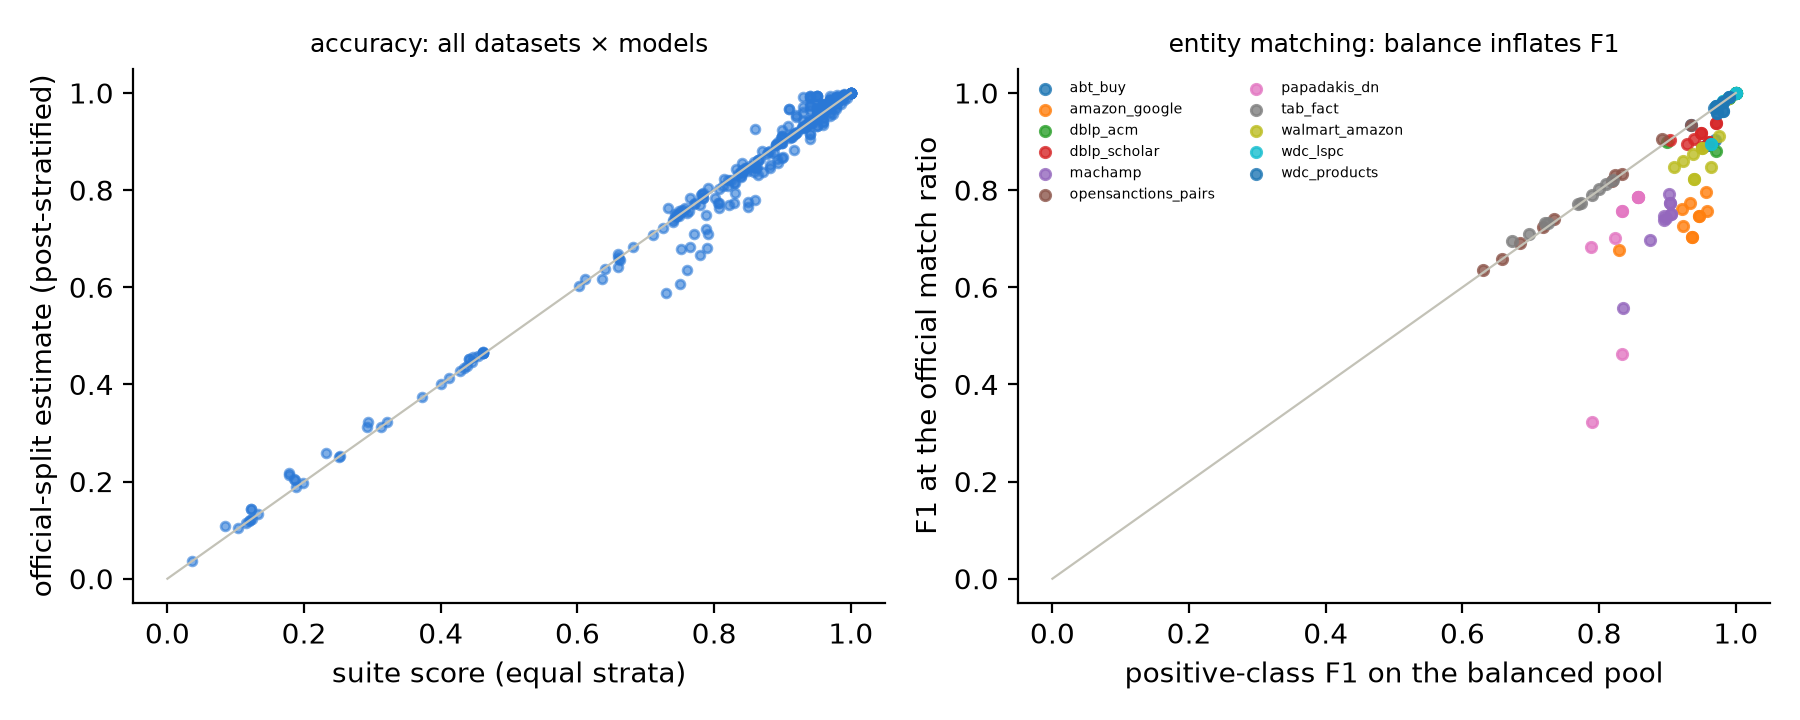
\includegraphics[width=0.9\textwidth]{fig_official_split.png}
\caption{Suite score vs post-stratified official estimate per dataset, and matching F1 on the balanced pool vs at the official match ratio.}
\label{fig:official}
\end{figure}
\notable{Almost every (dataset, model) point lies on the diagonal for accuracy; the sparse matching sets fall below it for F1. Model order is preserved after re-weighting; the absolute numbers are not, so the official-ratio column is the one to compare with published results.}

\subsection{Dataset diagnostics}
\inoneline{Three sets are at ceiling and twelve separate no model pair; a dozen table and document sets carry the result.}
Three datasets sit at ceiling (mean composite 0.98 with a spread of 0.02--0.04 across models): Valentine, WDC LSPC and WDC Products. They are flagged and remain inside the objective in this run. Two sit near floor for every model (OfficeQA closed-book and OfficeQA Pro V2) and one is a known hard set (BIRD); none is excluded. Self-stability $\tau$ (rank agreement between bootstrap halves of a dataset) ranges from 0.57 to 0.92. Twelve datasets, all the entity-matching sets plus Valentine and TPC-DI, separate no model pair at the item level; four separate twenty or more.

\end{document}
